\documentclass[11pt]{article}
%Gummi|065|=)
\title{\textbf{Meccano pentagons}}
\author{https://github.com/heptagons/meccano/penta}
\date{}

\usepackage{amsmath}
\usepackage[pdftex]{graphicx}
\usepackage{listings}
\usepackage{xcolor}
\definecolor{gray}{RGB}{245,245,245}

\lstset{
	backgroundcolor=\color{gray},
	frame=single,
	numbers=left,
	stepnumber=1,
	tabsize=2,
	basicstyle=\ttfamily\small,
	breaklines=true
}

\usepackage[margin=0.75in]{geometry}

\usepackage{graphicx}
\usepackage{hyperref}
\begin{document}

\maketitle
\begin{abstract}
We show how to construct two types of meccano\footnote{
\href{https://webspace.science.uu.nl/~hooft101/lectures/meccano.pdf}{Meccano mathematics by `t Hooft }
}
regular pentagons.
The process as in another meccano constructions of this site is to build
the polygon perimeter and attach \textbf{internal diagonals} to make the polygon rigid.

We prepare general layouts to look for the use of only valid \textbf{meccano rods} testing 
by increasing the sides lengths and by rotating the diagonals.

The last diagonal most of the time is not an integer, so the purpose of this study is to find
when it is as the rest of diagonals and tabulate a so called solution. Formulas are
prepared exactly for each type instead of using floating numbers to prevent skip solutions by
rounding errors. Finally a program is run using the algebraic conditions and formulas
to iterate over a given range of sides to store and print solutions without repetitions by scaling.
\newline\newline
From the two types of pentagons two conjectures emerges. \textbf{First conjecture} is
that the first type of pentagon seems to have a \textbf{unique} solution after testing
pentagons sides somehow large.
\newline\newline
\textbf{Second conjecture} appears in second type of pentagon. For this type we got a lot of solutions 
but by inspecting the numeric value of the last diagonal called $e$ seems to be always in the form
\textbf{$10x + 1$} for $x = 1,2,3..$ something unrelated at the moment by the formulas used.
\end{abstract}

\section{Regular pentagon type 1}

\begin{figure}[htpb]
\centering
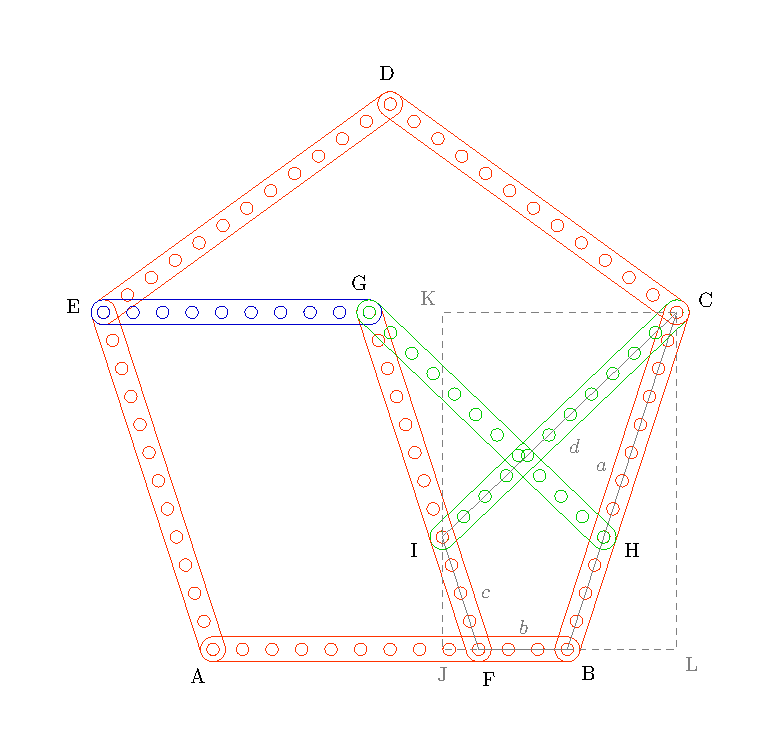
\includegraphics[scale=1]{penta-type-1}
\caption{Pentagon of type 1.}
\label{fig:type-1}
\end{figure}

\subsection{Type 1 equations}

Figure \ref{fig:type-1} show the layout of the meccano regular pentagon of type 1.
Let define the side of the pentagon as $a$ and define other three variables $b$, $c$ and $d$:
\begin{align*}
a &= \overline{BC}\\
b &= \overline{BF}\\
c &= \overline{FI}\\
d &= \overline{CI}
\end{align*}

Angles $\angle{LBC}$ and $\angle{JFI}$ are equal to $\frac{2\pi}{5}$ so:
\begin{align*}
\alpha &= \frac{2\pi}{5}\\
\overline{BL} &= a\cos{\alpha}\\
\overline{CL} &= a\sin{\alpha}\\
\overline{FJ} &= c\cos{\alpha}\\
\overline{IJ} &= c\sin{\alpha}
\end{align*}

Let calculate $d$ in function of $a$, $b$ and $c$:
\begin{align*}
d^2 &= (\overline{CI})^2\\
    &= (\overline{CK})^2 + (\overline{IK})^2\\
    &= (\overline{BL} + \overline{BF} + \overline{FJ})^2 + (\overline{CL} - \overline{IJ})^2\\
    &= (a\cos{\alpha} + b + c\cos{\alpha})^2 + (a\sin{\alpha} - c\sin{\alpha})^2\\
    &= ((a+c)\cos{\alpha} + b)^2 + ((a-c)\sin{\alpha})^2\\
    &= (a+c)^2\cos^2{\alpha} + 2(a+c)b\cos{\alpha} + b^2 + (a-c)^2\sin^2{\alpha}\\
    &= (a^2+c^2)(cos^2{\alpha}+sin^2{\alpha}) + 2ac(cos^2{\alpha}-\sin^2{\alpha})+ 2(a+c)b\cos{\alpha} + b^2\\
    &= (a^2+c^2) + 2ac(cos^2{\alpha}-\sin^2{\alpha})+ 2(a+c)b\cos{\alpha} + b^2\\
\end{align*}

For $\alpha = \frac{2\pi}{5}$ we have these regular pentagon identities:
\begin{align*}
cos{\alpha}   &= \frac{-1 + \sqrt{5}}{4} \\
cos^2{\alpha} &= \frac{{ 3 - \sqrt{5}}}{8} \\
sin^2{\alpha} &= \frac{5 + \sqrt{5}}{8} \\
cos^2{\alpha} - sin^2{\alpha} &= -\frac{1 + \sqrt{5}}{4}
\end{align*}

Applying the identities to the last equation of $d$ we get:
\begin{align*}
d^2 &= a^2 + c^2 - (\frac{1 + \sqrt{5}}{2})ac + (\frac{-1 + \sqrt{5}}{2})(a+c)b + b^2\\
    &= a^2 + c^2 - \frac{ac}{2} - \frac{(a+c)b}{2} + b^2 + [- \frac{ac}{2} + \frac{(a+c)b}{2}]\sqrt{5}\\
    &= a^2 + b^2 + c^2 - \frac{ac + (a+c)b}{2} + [\frac{-ac + (a+c)b}{2}]\sqrt{5}
\end{align*}

Let define two variables $p$ and $q$ such that $d^2 = p + q\sqrt{5}$ so we have:
\begin{align*}
d^2 &= p + q\sqrt{5}\\
  q &= \frac{-ac + (a + c)b}{2}\\
  p &= a^2 + b^2 + c^2 - \frac{ac + (a+c)b}{2}\\
    &= a^2 + b^2 + c^2 - \frac{-ac + (a+c)b}{2} - ac\\
    &= a^2 + b^2 + c^2 - q - ac
\end{align*}

For a meccano pentagon we need $d$ to be an integer. If we let the integer $q > 0$ then $d = \sqrt{p + q\sqrt{5}}$ will never be an integer for $p$ and $q$ integers. If we force $q$ to be zero then $d = \sqrt{p}$ has possibilities to be an integer.
So before calculating $d$ we force the condition that $q = 0$ or that is the same $-ac + (a+c)b = 0$:
\begin{align*}
a  & > b\\
a  & > c\\
ac &= (a + c)b\\
 d &= \sqrt{a^2 + b^2 + c^2 + ac}
\end{align*}

\subsection{Type 1 program}

First we write a \textbf{go} struct called \texttt{Sols} to collect and print solutions found for the following searchinv function of any pentagon type. The struct \texttt{Add} function prevent
solutations duplicated by scaling:
\begin{lstlisting}
type Sols struct {
	sols [][]int
}

func (s *Sols) Add(rods ...int) {
	if len(rods) < 0 {
		return
	}
	const RODS = "abcdefhijkl"
	for _, s := range s.sols {
		a := rods[0]
		if a % s[0] != 0 { 
			continue
		}
		// new a is a factor of previous a
		f := a / s[0]
		cont := false
		for r := 1; r < len(rods); r++ {
			if s[r] == 0 {
				continue
			}
			b := rods[r]
			if t := b % s[r] == 0 && b / s[r] == f; !t {
				cont = true
				break
			}
		}
		if cont {
			continue // scaled solution already found (reject)
		}
		return
	}
	// solution!
	if s.sols == nil {
		s.sols = make([][]int, 0)
	}
	s.sols = append(s.sols, rods)
	fmt.Printf("%3d ", len(s.sols))
	for i, r := range rods {
		fmt.Printf(" %c=%3d", RODS[i], r)
	}
	fmt.Println()
}

\end{lstlisting}

Next \textbf{go} function called \texttt{pentagons\_type\_1} iterate over three variables 
$a \leq max$, $1 \leq b \leq a$, $0 \leq c \leq a$ (lines 15, 16 and 17).
The $q = 0$ condition is tested (line 18) and only when is valid we check $d$ to be an integer (see internal function at line 5).
Only when $d$ is an integer we call function sorts Add (in line 11) to print and store a 
prospect of solution.
\begin{lstlisting}
func pentagons_type_1(max int) {

	sols := &Sols{}

	check := func(a, b, c int) {
		f := float64(a*a + b*b + c*c - a*c)
		if f < 0 {
			return
		}
		if d := int(math.Sqrt(f)); math.Pow(float64(d), 2) == f {
			sols.Add(a, b, c, d)
		}
	}

	for a := 1; a < max; a++ {
		for b := 1; b <= a; b++ {
			for c := 0; c <= a; c++ {
				if a*c == (a + c)*b {
					check(a, b, c)
				}
			}
		}
	}
}
}
\end{lstlisting}

\subsection{Type 1 results}
After serching for values of $a <= 5000$ we found a single result:

\begin{lstlisting}
  1  a= 12 b=  3 c=  4 d= 11
\end{lstlisting}

\begin{figure}
\centering
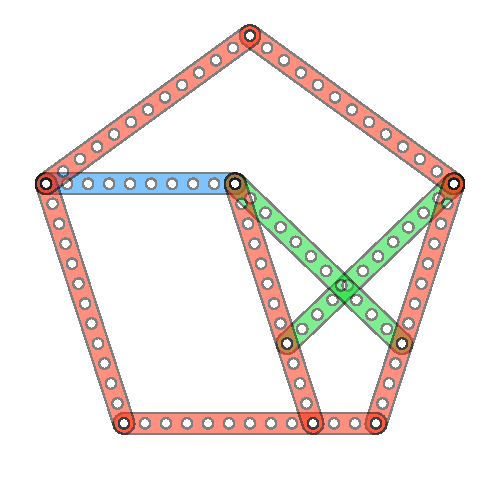
\includegraphics[width=7cm]{figs/pentagon-12a}
\caption{The smallest and maybe unique (?) of pentagons of type 1.
Is composed of 6 rods of length $a = 12$ in color red,
two rods of length $d=11$ in green and one rod of size $a-b = 9$ in blue.}
\label{pentagon-12a}
\end{figure}

Figure \ref{pentagon-12a} shows the first (unique?) pentagon of type 1 with values
$a=12$, $b=3$, $c=4$ and $d=11$.

\subsection{Type 1 conjecture}
There is only a single case for the type 1 with values $a=12$, $b=3$, $c=4$ and $d=11$.

%%%%%%%%%%%%%
\vspace{100em}

\section{Regular pentagon type 2}

\begin{figure}[htpb]
\centering
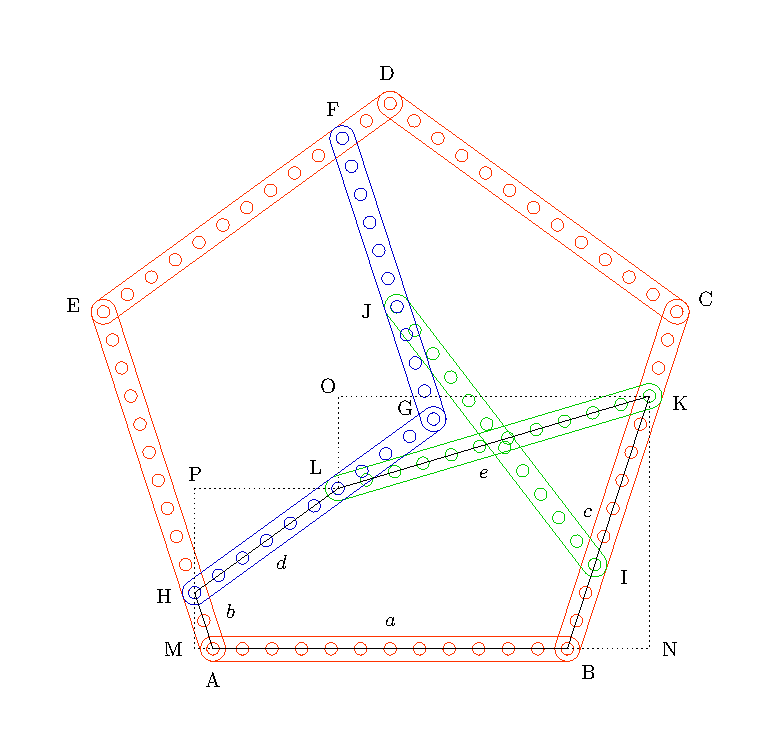
\includegraphics[scale=0.75]{penta-type-2}
\caption{Pentagon of type 2.}
\label{fig:type-2}
\end{figure}

\subsection{Type 2 equations}

Figure \ref{fig:type-2} show the layout of the meccano regular pentagon of type 2.
Let define the side of the pentagon as $a$ and define other four variables $b$, $c$, $d$ and $e$:
\begin{align*}
a &= \overline{AB}\\
b &= \overline{AH}\\
c &= \overline{BK}\\
d &= \overline{HL}\\
e &= \overline{KL}
\end{align*}

Angles $\angle{NBC}$ and $\angle{MAH}$ are equal to $\frac{2\pi}{5}$ so:
\begin{align*}
\alpha &= \frac{2\pi}{5}\\
\overline{BN} &= b\cos{\alpha}\\
\overline{KN} &= b\sin{\alpha}\\
\overline{AM} &= c\cos{\alpha}\\
\overline{HM} &= c\sin{\alpha}
\end{align*}

Angle $\angle{PLH}$ is equal to $\frac{\pi}{5}$ so:
\begin{align*}
\beta &= \frac{\pi}{5}\\
\overline{LP} &= d\cos{\beta}\\
\overline{HP} &= d\sin{\beta}
\end{align*}

Our goal is to find $e$ as integer as funcion of variables $a$, $b$, $c$ and $d$.
$e^2$ equals $(\overline{KO})^2 + (\overline{LO})^2$ so we first calculate 
$\overline{KO}$ and $\overline{LO}$. From figure \ref{fig:type-2}:
\begin{align*}
\overline{KO} &= \overline{AM} + \overline{AB} + \overline{BN} - \overline{LP}\\
              &= b\cos{\alpha} + a + c\cos{\alpha} - d\cos{\beta}\\
              &= (b+c)\cos{\alpha} + a  - d\cos{\beta}\\
\overline{LO} &= \overline{KN} - \overline{HM} - \overline{HP}\\
              &= c\sin{\alpha} - b\sin{\alpha} - d\sin{\beta}\\
              &= (c-b)\sin{\alpha} - d\sin{\beta}
\end{align*}

So by adding the squares we get:
\begin{align*}
e^2 &= (\overline{KO})^2 + (\overline{LO})^2\\
    &= ((b+c)\cos{\alpha})^2 + 2(b+c)\cos{\alpha}(a - d\cos{\beta}) + (a - d\cos{\beta})^2\\
    &\qquad + ((c-b)\sin{\alpha})^2 - 2(c-b)\sin{\alpha}d\sin{\beta} + (d\sin{\beta})^2\\
    &= (b^2+c^2)(cos^2{\alpha}+sin^2{\alpha}) + 2bc(cos^2{\alpha}-sin^2{\alpha})\\
    &\qquad + 2a(b+c)cos{\alpha} - 2(b+c)d\cos{\alpha}\cos{\beta} - 2(c-b)d\sin{\alpha}\sin{\beta}\\
    &\qquad + a^2 - 2ad\cos{\beta} + d^2(\cos^2{\beta} + \sin^2{\beta})
\end{align*}

Calculate the $\alpha$ and $\beta$ identities that appear in the last equation:
\begin{align*}
\cos^2{\alpha} - \sin^2{\alpha} &= -\frac{1 + \sqrt{5}}{4}\\
                   \cos{\alpha} &= \frac{-1+\sqrt{5}}{4}\\
        \cos{\alpha}\cos{\beta} &= \frac{1}{4}\\
        \sin{\alpha}\sin{\beta} &= \frac{\sqrt{5}}{4}\\
                    \cos{\beta} &= \frac{1+\sqrt{5}}{4}
\end{align*}

Replace the identities:
\begin{align*}
e^2 &= (b^2+c^2)(1) + 2bc(-\frac{1 + \sqrt{5}}{4})\\
    &\qquad + 2a(b+c)(\frac{-1+\sqrt{5}}{4}) - 2(b+c)d(\frac{1}{4}) - 2(c-b)d(\frac{\sqrt{5}}{4})\\
    &\qquad + a^2 - 2ad(\frac{1+\sqrt{5}}{4}) + d^2(1)\\
    %
    &= b^2+c^2 - bc(\frac{1 + \sqrt{5}}{2})\\
    &\qquad + a(b+c)(\frac{-1+\sqrt{5}}{2}) - (b+c)d(\frac{1}{2}) - (c-b)d(\frac{\sqrt{5}}{2})\\
    &\qquad + a^2 - ad(\frac{1+\sqrt{5}}{2}) + d^2\\
    %
    &= a^2+b^2+c^2 + d^2 - (b+c)d(\frac{1}{2}) \\
    &\qquad - (ad+bc)(\frac{1 + \sqrt{5}}{2}) + a(b+c)(\frac{-1+\sqrt{5}}{2}) - (c-b)d(\frac{\sqrt{5}}{2})\\
    &= a^2+b^2+c^2 + d^2 - \frac{(b+c)d}{2} \\
    &\qquad - \frac{(ad+bc)(1 + \sqrt{5})}{2} + \frac{a(b+c)(-1+\sqrt{5})}{2} - \frac{(c-b)d\sqrt{5}}{2}
\end{align*}

Let define two variables $p$ and $q$ such that $e^2 = p + q\sqrt{5}$:
\begin{align*}
p &= a^2+b^2+c^2 + d^2 - \frac{(b+c)d}{2} - \frac{ad+bc}{2} + \frac{-a(b+c)}{2}\\
  &= a^2+b^2+c^2 + d^2 - \frac{bd +cd +ad +bc +ab + ac}{2}\\
  &= a^2+b^2+c^2 + d^2 - \frac{(a+b)(c+d)+ab+cd}{2}\\
q &= - \frac{ad+bc}{2} + \frac{a(b+c)}{2} - \frac{(c-b)d}{2}\\
  &= \frac{-ad - bc + ab + ac - cd + bd}{2}\\
  &= \frac{(a-b)(c-d) + ab - cd}{2}
\end{align*}

For a meccano pentagon we need $e$ to be an integer. If we let the integer $q > 0$ then $e = \sqrt{p + q\sqrt{5}}$ will never be an integer for $p$ and $q$ integers. If we force $q$ to be zero then $e = \sqrt{p}$ has possibilities to be an integer.
So before calculating $e$ we force the condition that $q = 0$ or that is the same $cd = (a-b)(c-d)+ab$:
\begin{align*}
a  & > b\\
a  & > c\\
cd &= (a-b)(c-d)+ab\\
\end{align*}

From the condition $q=0$ we know that $cd = (a-b)(c-d)+ab$, and use this $cd$ value in 
in the equation for $p$ to get:
\begin{align*}
p &= a^2+b^2+c^2+d^2 - \frac{(a+b)(c+d)+ab+cd}{2}\\
  &= a^2+b^2+c^2+d^2 - \frac{(a+b)(c+d)+ab+(a-b)(c-d)+ab}{2}\\
  &= a^2+b^2+c^2+d^2 -ac -bd -ab
\end{align*}

So finally, when $q=0$ we calculate $e = \sqrt{p}$ expecting to be an integer:
\begin{align*}
e &= \sqrt{a^2 + b^2 + c^2 + d^2 -ac -bd - ab}
\end{align*}

Another solution is:
\begin{align*}
e &= \sqrt{a^2 + b^2 + c^2 + d^2 -ad -bc - cd}
\end{align*}


\subsection{Type 2 first program}

With the last equations, next go function search for solutions of type 2.
Is called \texttt{pentagons\_type\_2}, iterates over the integer values of rods 
$a$ (line 15), $b$ (line 16), $c$ (line 17) and $d$ (line 18)
to discover a rod $e$ with integer length too. First we check condition $q == 0$ is
true (line 19) and square root is integer (line 10):
\begin{lstlisting}
func pentagons_type_2(max int) {

	sols := &Sols{}

	check := func(a, b, c, d int) {
		f := float64(a*a + b*b + c*c + d*d - a*c - b*d - a*b)
	    if f < 0 {
	    	return
	    }
		if e := int(math.Sqrt(f)); math.Pow(float64(e), 2) == f {
			sols.Add(a, b, c, d, e)
		}
	}

    for a := 1 ; a < max; a++ {
    	for b := 1; b < a; b++ {
        	for c := 0; c < a; c++ {
          		for d := 1; d < a; d++ {
            		if ((a - b)*(c - d) + a*b == c*d) {
              			check(a, b, c, d)
              		}
              	}
            }
        }
    }
}
\end{lstlisting}

\subsection{Type 2 first results}
The program found 19 pentagons of type 2 for $a \leq 100$.
While we found a single solution for type 1, type 2 has several.

\begin{lstlisting}
  1  a= 12 b=  2 c=  9 d=  6 e= 11
  2  a= 12 b=  3 c=  0 d=  4 e= 11
  3  a= 12 b=  6 c=  3 d= 10 e= 11
  4  a= 31 b=  4 c= 28 d= 16 e= 31
  5  a= 31 b= 15 c=  3 d= 27 e= 31
  6  a= 38 b= 12 c= 18 d= 21 e= 31
  7  a= 38 b= 17 c= 20 d= 26 e= 31
  8  a= 48 b=  8 c= 24 d= 21 e= 41
  9  a= 48 b= 12 c=  9 d= 20 e= 41
 10  a= 48 b= 27 c= 24 d= 40 e= 41
 11  a= 48 b= 28 c= 39 d= 36 e= 41
 12  a= 72 b= 21 c= 48 d= 40 e= 61
 13  a= 72 b= 24 c= 16 d= 39 e= 61
 14  a= 72 b= 32 c= 24 d= 51 e= 61
 15  a= 72 b= 33 c= 56 d= 48 e= 61
 16  a= 78 b= 27 c=  4 d= 42 e= 71
 17  a= 78 b= 36 c= 74 d= 51 e= 71
 18  a= 87 b= 28 c= 36 d= 48 e= 71
 19  a= 87 b= 39 c= 51 d= 59 e= 71
\end{lstlisting}


\subsection{Type 2 simpler program}

\begin{figure}[htpb]
\centering
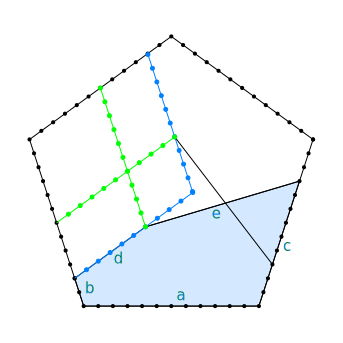
\includegraphics[scale=0.75]{figs/type-2-double}
\caption{Pentagon of type 2 has a symmetry where pair bars green and blue can be switched leaving
the bars $e$ lengths and positions unmodified. This symmetry appears in the first program when two solutions have same $a$ and same $e$.}
\label{fig:type-2-double}
\end{figure}

Figure \ref{fig:type-2-double} show what happens when the first program reports
two solutions with the same $a$ and the same $e$. 
The type 2 symmetry can be taken into account to simplify the first program
to reduce the search space and report only the half of symmetries.
Next go function called \texttt{pentagons\_type\_2\_half} first iterates
over $1 \leq a \leq max$ (line 4),
then over $1 \leq b < a$ (line 6),
then over $1 \leq d < (a-b)$ (line 8)
and finally over $0 \leq c < a$ (line 10).

\begin{lstlisting}
func pentagons_type_2_half(max int) {
	sols := &Sols{}
	aa, a_b, ab, bb, dd, ad, bc, c_d, cd, cc := 0,0,0,0,0,0,0,0,0,0
	for a := 1; a <= max; a++ {
		aa = a*a
		for b := 1; b < a; b++ {
			a_b, ab, bb = a - b, a*b, b*b
			for d := 1; d < (a-b); d++ {
				dd, ad = d*d, a*d
				for c := 0; c < a; c++ {
					bc, c_d, cd, cc = b*c, c - d, c*d, c*c
					if a_b * c_d + ab == cd {
						if f := float64(aa + bb + cc + dd - ad - bc - cd); f > 0 {
							if e := int(math.Sqrt(f)); math.Pow(float64(e), 2) == f {
								sols.Add(a, b, c, d, e)
							}
						}
					}
				}
			}
		}
	}
}
\end{lstlisting}

\subsection{Type 2 simpler results}
The secont type 2 program found $139$ solutions iterating over $1 \leq a \leq 1000$: 
\begin{lstlisting}
  1  a= 12 b=  2 c=  9 d=  6 e= 11
  2  a= 12 b=  3 c=  0 d=  4 e= 11
  3  a= 31 b=  4 c= 28 d= 16 e= 31
  4  a= 38 b= 12 c= 18 d= 21 e= 31
  5  a= 48 b=  8 c= 24 d= 21 e= 41
  6  a= 48 b= 12 c=  9 d= 20 e= 41
  7  a= 72 b= 21 c= 48 d= 40 e= 61
  8  a= 72 b= 24 c= 16 d= 39 e= 61
  9  a= 78 b= 27 c=  4 d= 42 e= 71
 10  a= 87 b= 28 c= 36 d= 48 e= 71
 11  a=111 b= 39 c= 99 d= 67 e=101
 12  a=121 b= 33 c= 33 d= 57 e=101
 13  a=128 b=  8 c= 89 d= 56 e=121
 14  a=138 b= 12 c= 54 d= 47 e=121
 15  a=145 b= 45 c= 39 d= 75 e=121
 16  a=147 b= 43 c= 51 d= 75 e=121
 17  a=151 b= 19 c= 73 d= 61 e=131
 18  a=156 b= 43 c= 96 d= 84 e=131
 19  a=165 b= 36 c=132 d= 88 e=151
 20  a=179 b= 15 c=177 d= 93 e=191
 21  a=183 b= 66 c= 62 d=108 e=151
 22  a=201 b=  9 c= 13 d= 21 e=191
 23  a=204 b= 21 c=112 d= 84 e=181
 24  a=216 b= 48 c=111 d=104 e=181
 25  a=236 b= 80 c= 20 d=125 e=211
 26  a=249 b= 45 c= 75 d= 95 e=211
 27  a=264 b= 76 c=  3 d=108 e=241
 28  a=285 b= 73 c= 27 d=111 e=251
 29  a=296 b=104 c=128 d=173 e=241
 30  a=303 b= 51 c= 29 d= 81 e=271
 31  a=304 b= 76 c=133 d=148 e=251
 32  a=312 b= 36 c= 93 d=100 e=271
 33  a=315 b= 24 c=160 d=120 e=281
 34  a=324 b= 64 c=204 d=159 e=281
 35  a=343 b=  7 c=115 d= 91 e=311
 36  a=352 b=  3 c=240 d=144 e=341
 37  a=354 b= 53 c= 60 d=102 e=311
 38  a=368 b= 36 c=219 d=156 e=331
 39  a=369 b= 37 c= 27 d= 63 e=341
 40  a=370 b=  1 c=172 d=118 e=341
 41  a=375 b= 15 c=191 d=135 e=341
 42  a=378 b= 21 c= 84 d= 86 e=341
 43  a=384 b=120 c=312 d=223 e=341
 44  a=390 b= 84 c= 50 d=135 e=341
 45  a=390 b= 87 c=228 d=194 e=331
 46  a=392 b=119 c=296 d=224 e=341
 47  a=392 b=128 c= 56 d=203 e=341
 48  a=393 b= 98 c= 54 d=156 e=341
 49  a=396 b=138 c= 73 d=222 e=341
 50  a=399 b= 70 c=210 d=180 e=341
 51  a=403 b= 78 c=114 d=156 e=341
 52  a=404 b= 89 c=104 d=164 e=341
 53  a=408 b= 16 c=312 d=183 e=401
 54  a=408 b= 84 c=167 d=180 e=341
 55  a=411 b=123 c=243 d=227 e=341
 56  a=435 b= 96 c=400 d=240 e=421
 57  a=450 b= 92 c=438 d=249 e=451
 58  a=468 b=173 c= 24 d=276 e=431
 59  a=480 b= 80 c= 75 d=144 e=421
 60  a=486 b=180 c= 18 d=287 e=451
 61  a=488 b= 72 c= 15 d= 96 e=451
 62  a=488 b=132 c=423 d=276 e=451
 63  a=488 b=152 c=269 d=272 e=401
 64  a=495 b=135 c=415 d=279 e=451
 65  a=502 b= 93 c= 36 d=138 e=451
 66  a=507 b= 18 c=366 d=220 e=491
 67  a=507 b= 60 c= 84 d=128 e=451
 68  a=509 b=150 c= 42 d=228 e=451
 69  a=516 b=114 c=169 d=222 e=431
 70  a=520 b= 36 c=225 d=180 e=461
 71  a=525 b=185 c=399 d=315 e=451
 72  a=525 b=189 c=105 d=305 e=451
 73  a=528 b= 80 c=171 d=192 e=451
 74  a=540 b=150 c=321 d=290 e=451
 75  a=543 b=123 c=221 d=249 e=451
 76  a=546 b=135 c=228 d=262 e=451
 77  a=552 b=179 c=288 d=312 e=451
 78  a=553 b=180 c=276 d=312 e=451
 79  a=560 b=200 c=344 d=335 e=461
 80  a=565 b= 69 c=153 d=177 e=491
 81  a=588 b=104 c= 12 d=135 e=541
 82  a=600 b= 65 c=240 d=216 e=521
 83  a=600 b=120 c= 96 d=205 e=521
 84  a=617 b= 89 c=533 d=317 e=601
 85  a=632 b=113 c=152 d=224 e=541
 86  a=652 b= 58 c=235 d=214 e=571
 87  a=661 b=109 c= 37 d=157 e=601
 88  a=684 b=237 c=192 d=388 e=571
 89  a=699 b= 84 c=564 d=344 e=671
 90  a=701 b=254 c=698 d=428 e=671
 91  a=713 b=234 c=582 d=420 e=631
 92  a=715 b=211 c=655 d=415 e=671
 93  a=720 b=216 c=712 d=423 e=701
 94  a=724 b=147 c= 72 d=228 e=641
 95  a=728 b= 21 c=192 d=168 e=661
 96  a=729 b= 36 c=428 d=288 e=671
 97  a=732 b= 18 c=681 d=358 e=781
 98  a=732 b= 42 c=111 d=134 e=671
 99  a=744 b=228 c=155 d=372 e=631
100  a=746 b=164 c= 38 d=233 e=671
101  a=755 b=123 c=267 d=291 e=641
102  a=756 b= 69 c=168 d=196 e=671
103  a=762 b= 73 c=372 d=294 e=671
104  a=765 b= 30 c=354 d=260 e=691
105  a=777 b=234 c=118 d=372 e=671
106  a=781 b=108 c=348 d=312 e=671
107  a=784 b=192 c=189 d=336 e=661
108  a=800 b=164 c=263 d=332 e=671
109  a=804 b=177 c=272 d=348 e=671
110  a=805 b=202 c=238 d=364 e=671
111  a=810 b=276 c=510 d=475 e=671
112  a=819 b=136 c=216 d=288 e=701
113  a=824 b=276 c=363 d=468 e=671
114  a=826 b=315 c=420 d=510 e=671
115  a=840 b=196 c=777 d=468 e=811
116  a=845 b=285 c=465 d=489 e=691
117  a=859 b=130 c=502 d=388 e=751
118  a=861 b=126 c= 66 d=196 e=781
119  a=863 b=303 c=711 d=519 e=761
120  a=864 b= 24 c=349 d=264 e=781
121  a=873 b=137 c=453 d=381 e=751
122  a=879 b=231 c= 63 d=343 e=781
123  a=885 b=206 c=642 d=468 e=781
124  a=885 b=309 c= 13 d=477 e=821
125  a=892 b=112 c=196 d=259 e=781
126  a=896 b=144 c=528 d=411 e=781
127  a=896 b=332 c=725 d=548 e=781
128  a=904 b=328 c=640 d=547 e=761
129  a=905 b=161 c=185 d=305 e=781
130  a=912 b=168 c=507 d=424 e=781
131  a=915 b=135 c=345 d=349 e=781
132  a=928 b=319 c=232 d=520 e=781
133  a=938 b=252 c=270 d=441 e=781
134  a=947 b=306 c=558 d=540 e=781
135  a=948 b=342 c=589 d=570 e=781
136  a=949 b=273 c=495 d=507 e=781
137  a=960 b=195 c=760 d=504 e=881
138  a=961 b=249 c=633 d=513 e=821
139  a=987 b=350 c=594 d=588 e=811
\end{lstlisting}

\subsection{Type 2 conjecture}
The last report of 139 pentagons shows all $e$ values have the form $10x + 1$ for $x$ integer.
So the conjecture is that $e$ always is of the form $10x + 1$ for $x$ integer.

Next go function called \texttt{pentagons\_type\_2\_half\_with\_conjecture}
is an adaptation of the previous one and instead checking for a square root to be an integer,
only checks for $e^2 = (10x+1)^2$ for small $x > 1$.
The results of this program is exactly the same result of the
program checking the square root, up to $a \leq 1000$.
\begin{lstlisting}
func pentagons_type_2_half_with_conjecture(max int) {
	sols := &Sols{}
	aa, a_b, ab, bb, dd, ad, bc, c_d, cd, cc := 0,0,0,0,0,0,0,0,0,0
	for a := 1; a <= max; a++ {
		aa = a*a
		for b := 1; b < a; b++ {
			a_b, ab, bb = a - b, a*b, b*b
			for d := 1; d < (a-b); d++ {
				dd, ad = d*d, a*d
				for c := 1; c < a; c++ {
					bc, c_d, cd, cc = b*c, c - d, c*d, c*c
					if a_b * c_d + ab == cd {

						e2 := aa + bb + cc + dd - ad - bc - cd

						x := 1
						for {
							if e := 10*x + 1; e*e == e2 {
								sols.Add(a, b, c, d, e)
								break
							} else if e*e > e2 {
								break
							}
							x++
						}
					}
				}
			}
		}
	}
}

\end{lstlisting} 

\subsection{Type 2 examples}

Figures \ref{pentagons-2-31}, \ref{pentagons-2-38} and \ref{pentagons-2-48} show some of the pentagons of type 2 found.

\begin{figure}
\centering
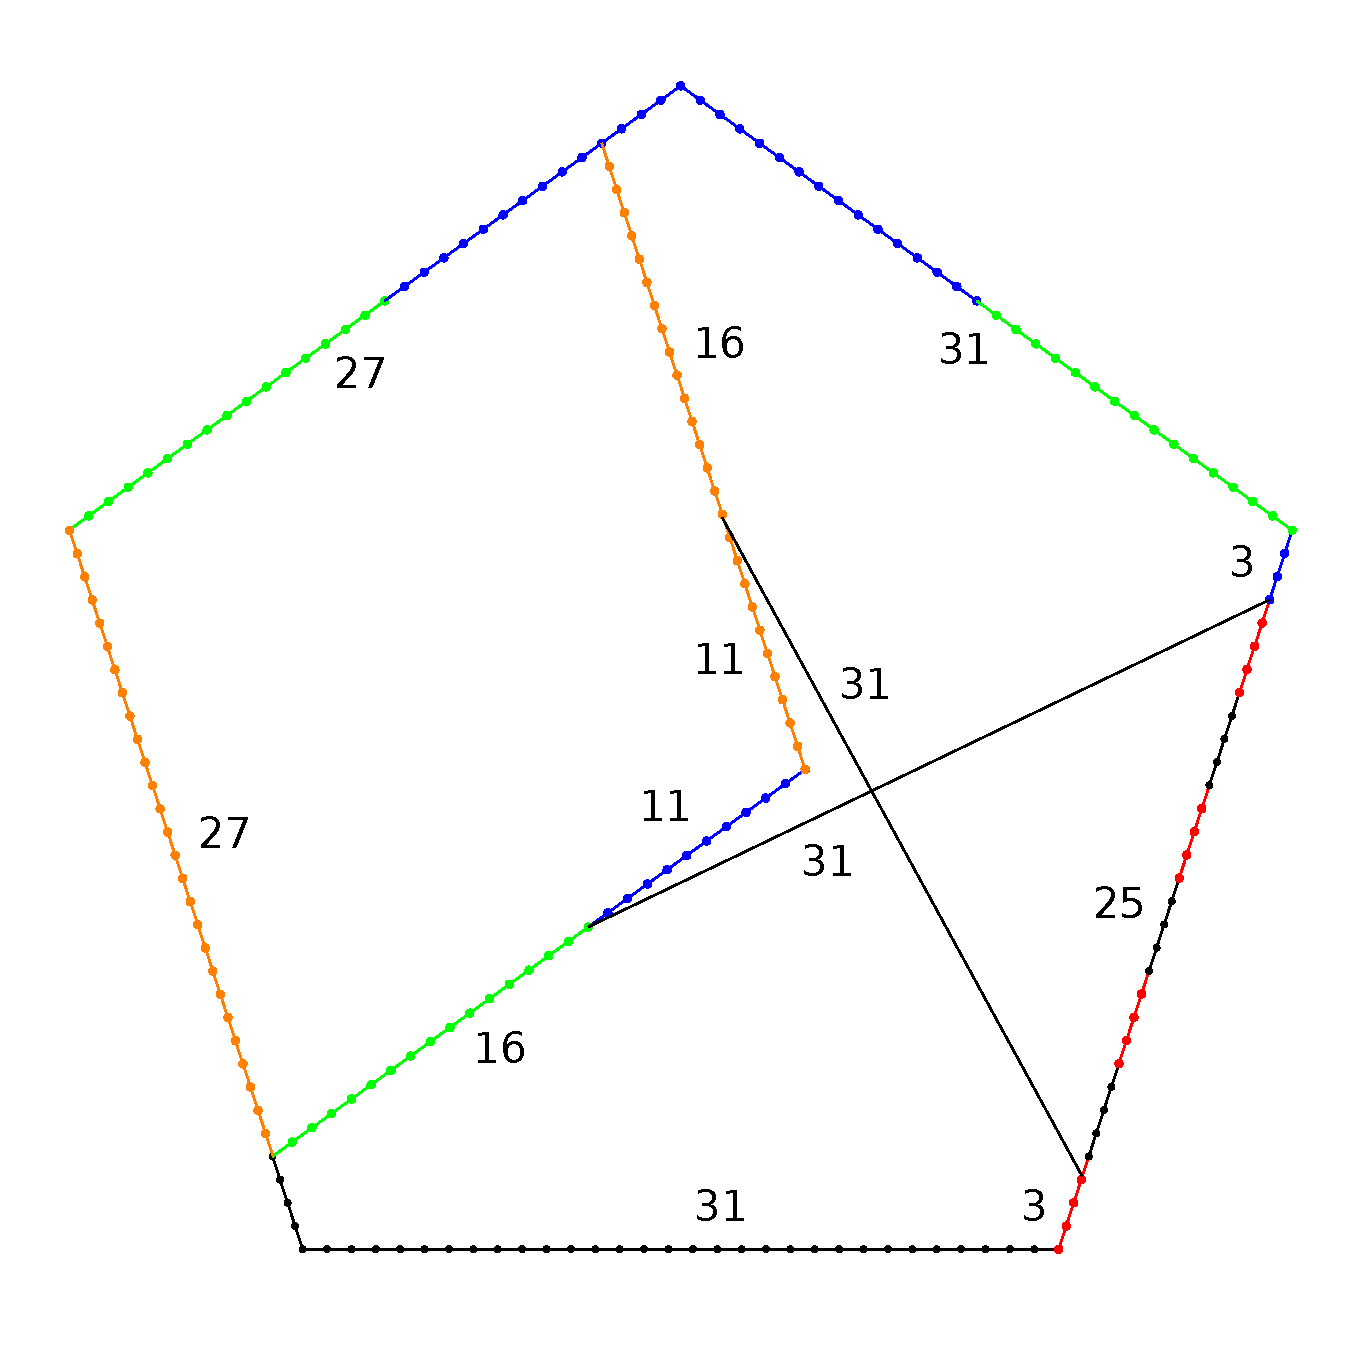
\includegraphics[width=10cm]{figs/pentagons-2-31}
\caption{Pentagon of type 2 with $a=31$. This construction requires 7 rods of 
length 31 and 2 rods of length 27.}
\label{pentagons-2-31}
\end{figure}

\begin{figure}
\centering
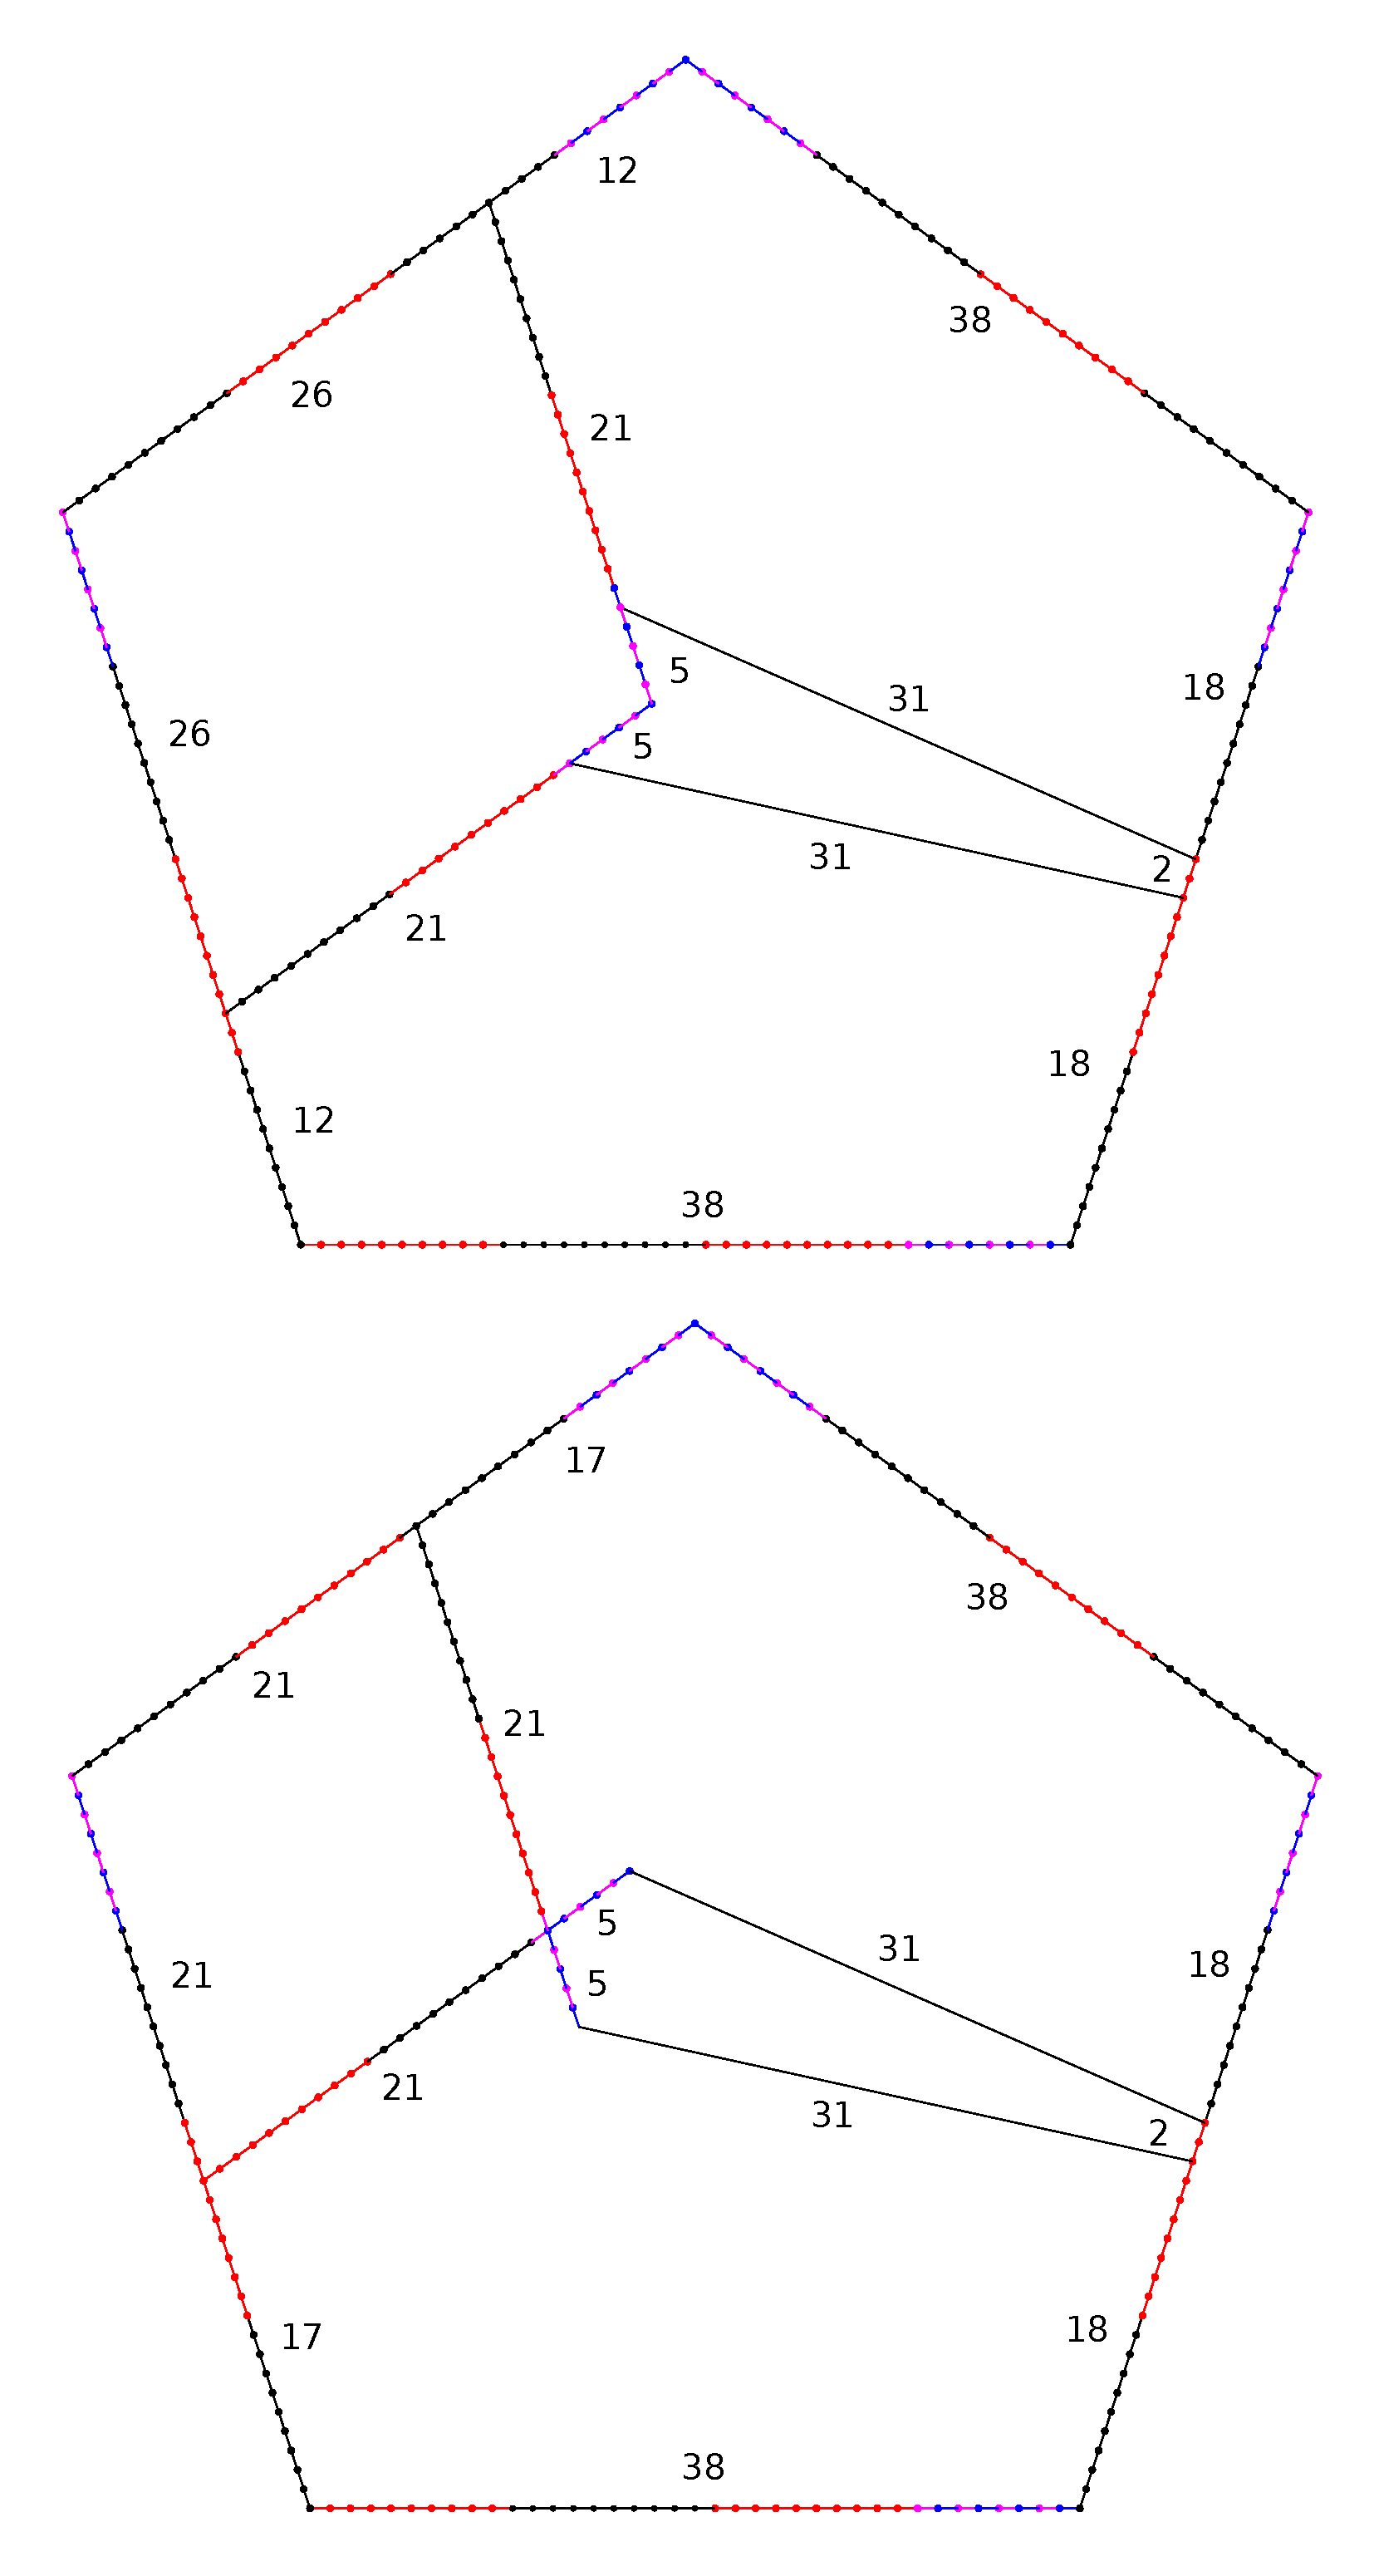
\includegraphics[width=10cm]{figs/pentagons-2-38}
\caption{Pentagons of type 2 with $a=38$. Each construction requires 5 rods
of length 38, 2 rods of length 31 and 2 rods of length 26}
\label{pentagons-2-38}
\end{figure}

\begin{figure}
\centering
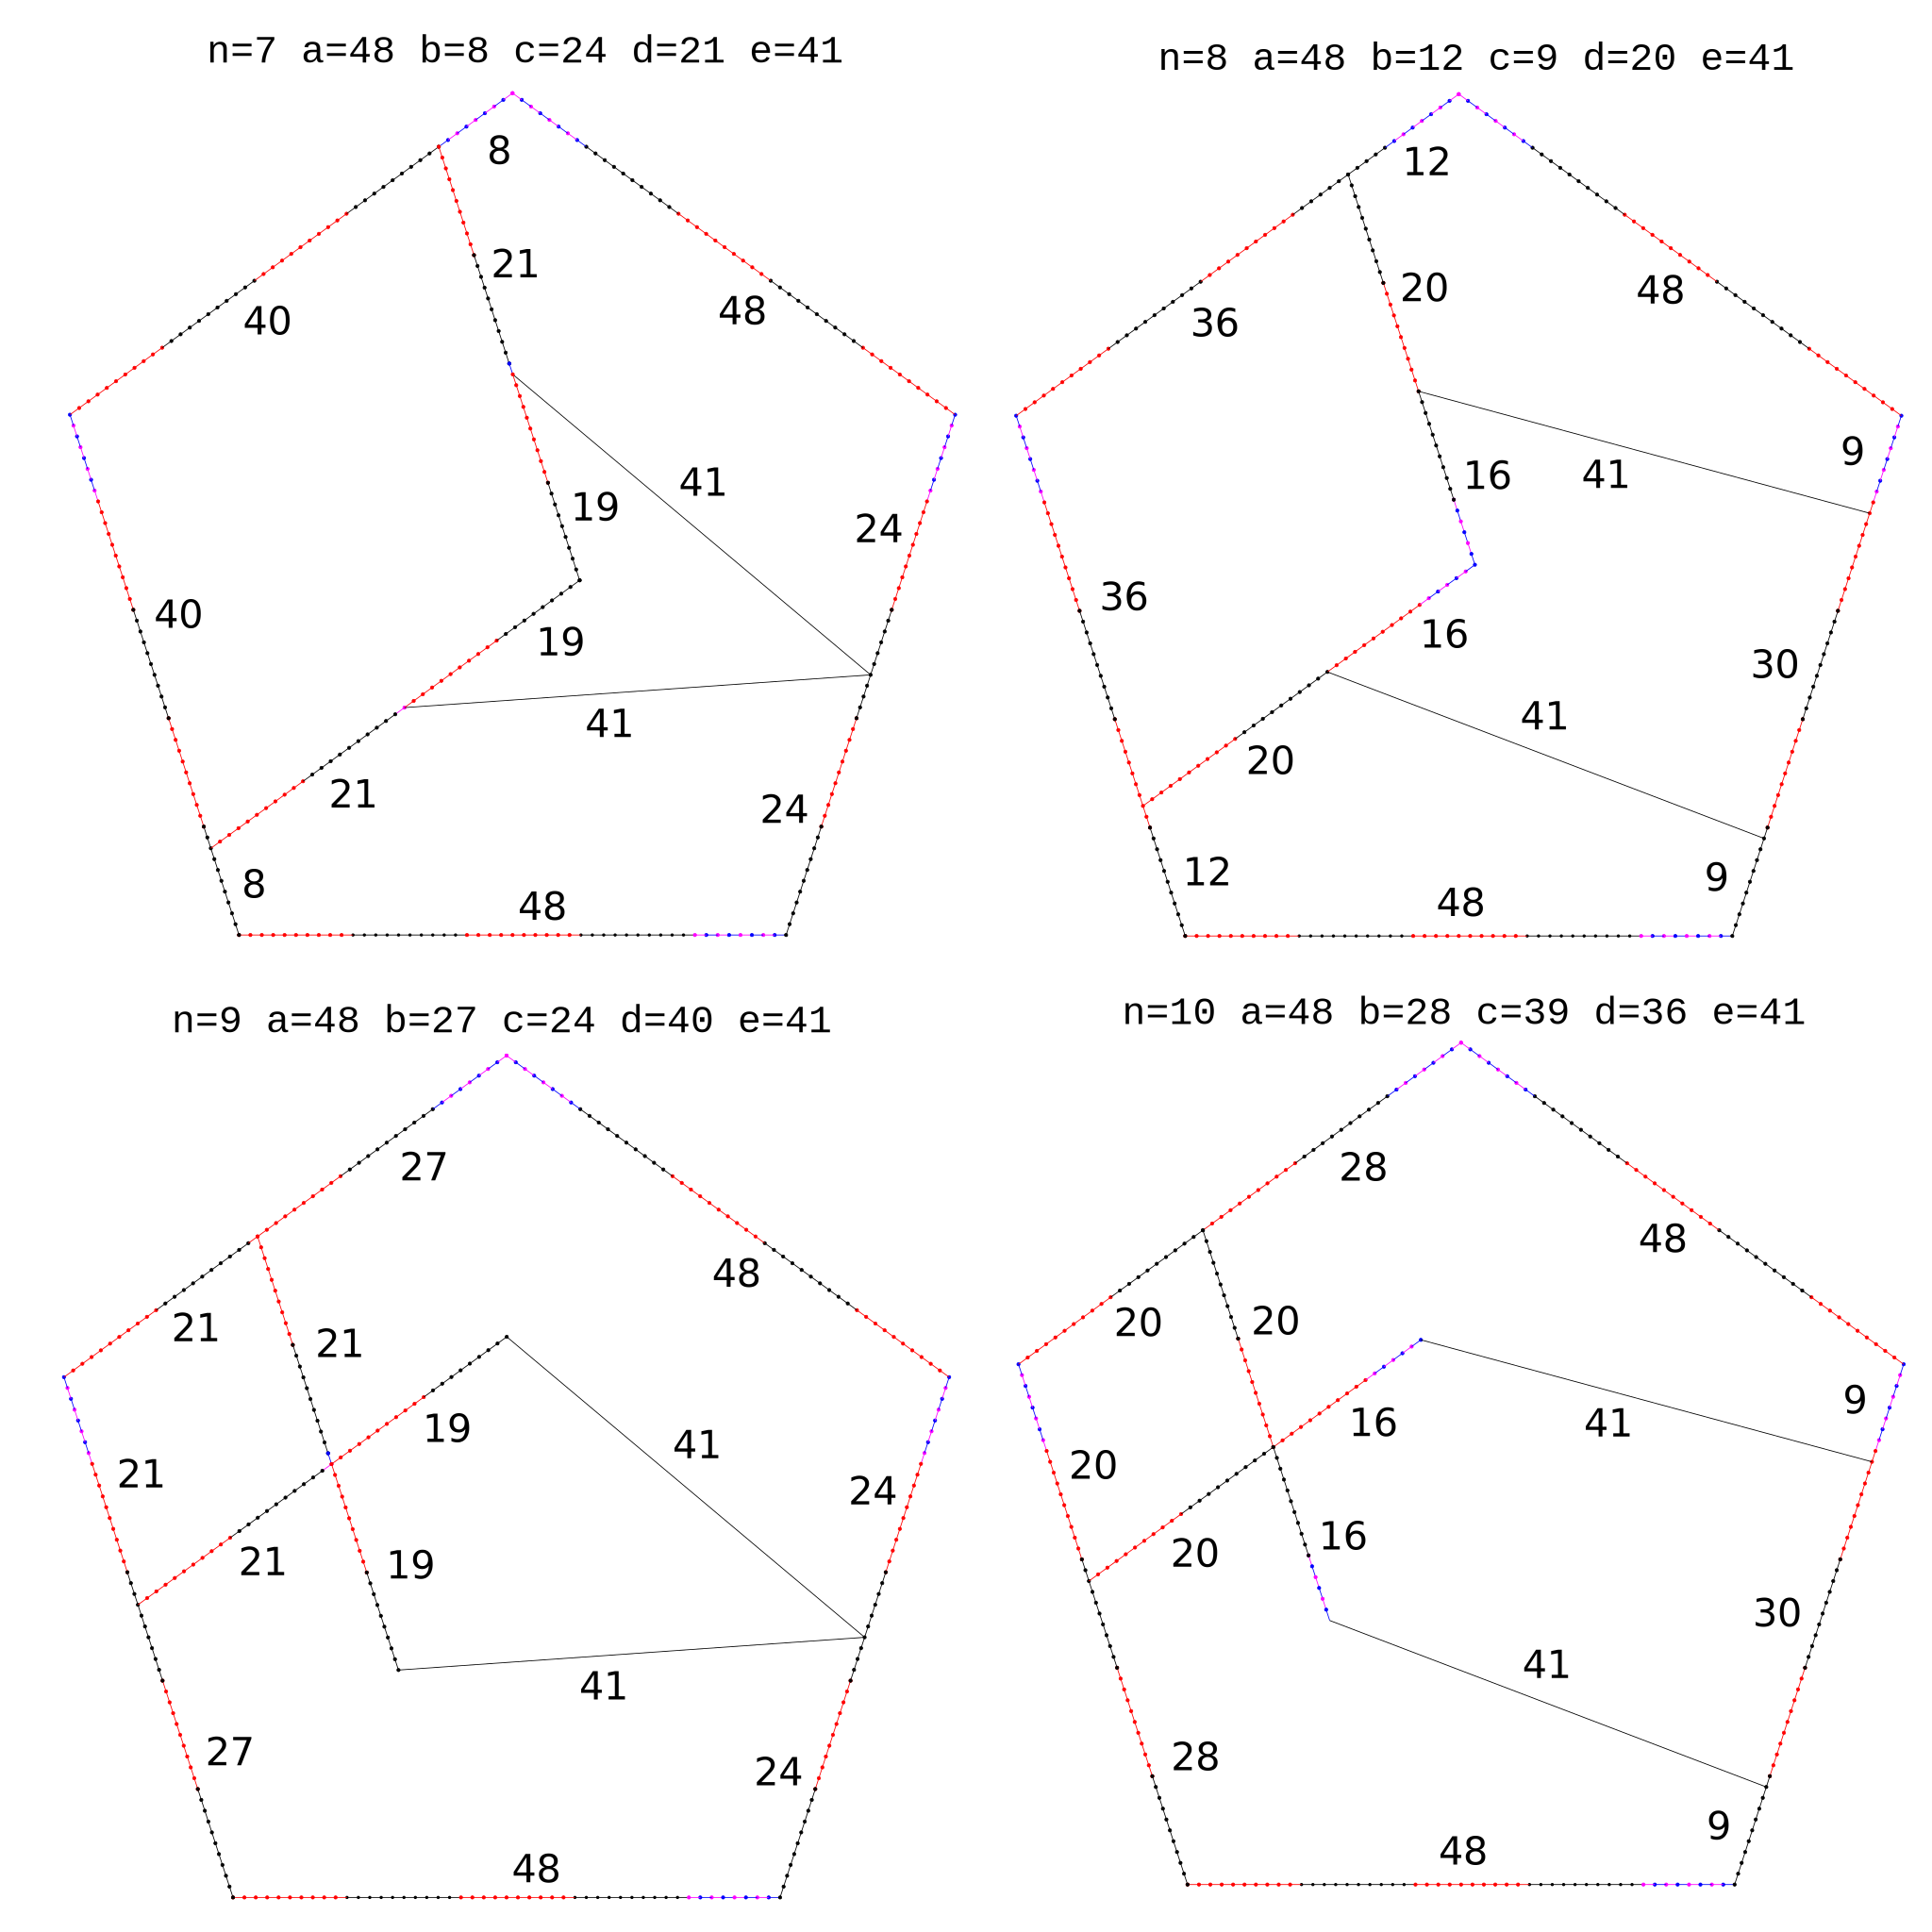
\includegraphics[width=15cm]{figs/pentagons-2-48}
\caption{Pentagons of type 2 with $a=48$}
\label{pentagons-2-48}
\end{figure}




\end{document}
